\documentclass{amsart}
\usepackage{amsfonts}
\usepackage[letterpaper,dvips,top=1.75in,left=1.75in,,right=1.75in,,
    foot=1in,,bottom=1.75in,]{geometry}
%\usepackage{times}
\usepackage{color}
\usepackage{hyperref}
\usepackage{graphicx}
\usepackage[T1]{fontenc}
\usepackage[charter]{mathdesign}
\usepackage{eulervm}
\usepackage{enumitem}
\usepackage{xcolor}

\newcommand{\tab}{\hspace*{2em}}

\begin{document}
\Large

\begin{flushleft}
{{\Large {Afton Geil \& Calina Copos \\[0pt]
\textbf{Project Report} \\[0pt]
EEC277 03/18/2012} \\[2pt]}}
\end{flushleft} 

\vspace{5mm}

\begin{center} {\LARGE {\textbf{Voxel-Based Screen Space Ambient Occlusion}} \\[5pt]}
\end{center}

\vspace{4mm}

\section{Introduction}

\indent{One of the biggest challenges in photorealistic rendering is calculating realistic lighting effects. Real world lighting is created by the interaction of photons with objects. We perceive an object when photons emitted from a light source hit an object, bounce off, then reach our eyes. Ray-tracing methods most closely approximate this by tracing the path from each point in the scene back to the camera. This results in very realistic-looking scenes, but it is very slow. In real-time computer graphics, lights are generally modeled either as directional or ambient. Directional lighting travels in one direction and originates at some source that may be within the field of view or a a distant point outside of the field of view. Ambient light accounts for the many times that light bounces off different objects so that objects that do not directly face the light source are still illuminated. Ambient lighting is generally modeled as isotropic lighting that originates at every point in space. For directional lighting, shadows are used to darken the areas that are blocked from interaction with the light. When objects are close to each other, they can also block some of the ambient light. Ambient occlusion accounts for this effect, resulting in a much more realistic scene.}

\indent{The basic principle behind ambient occlusion methods is to look at each point and determine what fraction of the surrounding volume is filled. The point is then darkened by an amount proportional to this value. Computing this volumetric integral can be rather complicated; however, we believe voxelization can simplify this calculation. Voxelization involves rendering a scene by breaking all of the objects up into volumetric elements, called voxels, rather the using triangle meshes to approximate the shape of an object. Approximating the integral as a sum of these elements should simplify the volume calculations, hopefully resulting in a faster overall rendering of the scene.}

\vspace{2mm}

\section{Related Work}

\indent{Ambient occlusion techniques are grouped into two types: object-space methods, which operate over all points, and screen-space methods, which operate only over points that are visible in the final image. For complex scenes, object-space methods are very expensive and are not practical for real-time applications. The first implementation of screen-space ambient occlusion was in \emph{Crysis} [1]. In this implementation, the Z-buffer was the only input needed to calculate the ambient occlusion. For each pixel in the scene, surrounding pixels are tested to determine whether they are in front of the pixel in question. The occlusion values are then weighted by their distance from the pixel in question, then added to produce the final ambient occlusion value.}

\indent{McGuire [2] computes what he calls "ambient occlusion volumes" by forming a bounding volume of polygons around the pixel and combining the contributions of all fragments within this volume using an integral approximation developed by Baum, et al. [3]. McGuire achieves visually appealing results with his algorithm, but the computation cannot be accomplished in real-time. The work most relevant to our proposed work is the work by Penmatsa and Wyman [4]. They compute ambient occlusion using voxels and sum up the contribution of each voxel face. They also measure the curvature of objects and use this for multiresolution effects, which they implement using mipmaps. Their solution runs at 40fps, but the quality of the images diverges considerably from ground truth.}

\vspace{2mm}

\section{Analytic Volumetric Occlusion}

Let X be an infinitesimal smooth patch $X$, and without loss of generality let the center be at the origin with normal $\hat{n}$. Ambient illumination is the incident light on $X$, due to objects outside of the patch.  Let $P$ be a voxel with vertices $\{\ \hat{p_0}, \hat{p_1} , ..., \hat{p_7}\}$, and let $\hat{c_0}$ be the centroid of the voxel with normal $\hat{N}$. The occlusion by $P$ of ambient light directed to $X$ is equal to the form factor that describes the diffuse radiative transfer between $P$ and $X$ as shown below:
\[ AO_P (\hat{n}) = \frac{1}{2\pi} \frac{\cos(\theta_P) \cdot \cos(\theta_X)}{r^2} A_P\]
where $\cos(\theta_P) = \hat{n} \cdot \psi$, $\cos(\theta_X) = \hat{N} \cdot \psi$, $\psi$ is the direction of the incoming radiance, $A_P$ denotes the screen projected volume of the voxel, and $r^2$ represents the squared distance between $c_0$ and $X$. We may interpret $\cos(\theta_P) \cdot \cos(\theta_X)$ as the amount of radiance reaching point $X$ depending on the angle made by $\psi$ with the normals of $c_0$ and $X$. The corrected integral approximation was first introduced by Baum et al. in the context of the radiosity algorithm [3].
\indent{}

\vspace{2mm}

\section{Ambient Occlusion Voxel Algorithm}

\indent{This project aims to introduce a new approximation algorithm for the voxel-based screen space ambient occlusion problem. It combines previous work to achieve substantially improved quality over fast methods and substantially improved performance compared to more accurate methods. The implementation of computing the analytic solution for ambient occlusion was written as a CUDA program while voxelization was implemented using an existing binary voxelization algorithm, binvox [5]. The main contribution of this project is an efficient algorithm for estimating ambient occlusion using an analytic solution to the integral form of the full matrix radiosity method.}

\begin{center}
\setlength\fboxsep{0pt}
\setlength\fboxrule{0.5pt}
\begin{figure}[htb]
\fbox{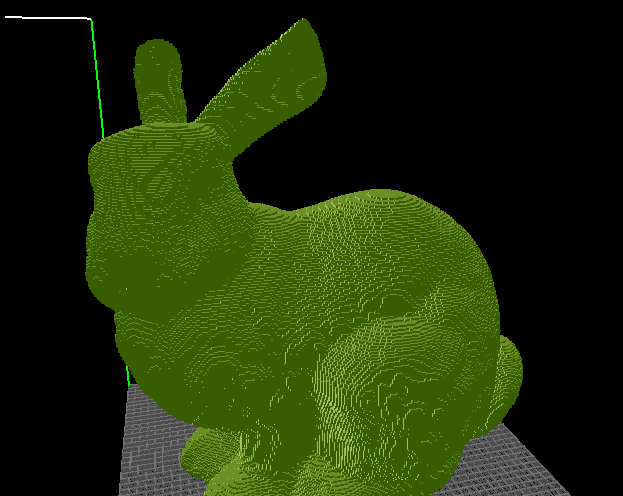
\includegraphics[scale=0.35]{voxel}}
\caption{Binary voxelized bunny scene using $256 \times 256 \times 256$ dicing planes in each direction. [5]}
\end{figure}
\end{center}

\fcolorbox{black}[HTML]{E9F0E9}{\parbox{\textwidth}{
\noindent \textbf{Preliminary ambient occlusion algorithm.}
\begin{enumerate}[nolistsep]
\item Render voxelized scene 
\item For each screen pixel:
		\item[-] Unproject to world space coordinates and then project to voxel space coordinates
		\item[-] Determine the position and normal of the centroid of voxels
		\item[-] Determine the neighborhood of occupied voxels and their relative distance
		\item[-] Use analytic solution to compute occlusion
		\item[-] Update occlusion buffer accordingly
\item Render the occlusion buffer
\end{enumerate}}}

\indent{}

\vspace{4mm}


\section*{References}

[1] Mittring, M.: "Finding next gen: Cryengine 2". In: ACM SIGGRAPH 2007 Courses, pp. 97--121 (2007).


[2] McGuire, M.: "Ambient Occlusion Volumes". In: Proceedings of High Performance Graphics, pp. 47-56 (2010).


[3] Baum, D., Rushmeier, H., Winget, J.: "Improving Radiosity Solutions Through the Use of Analytically Determined Form-Factors." Computer Graphics 23(3), pp. 325--334 (1989).


[4] Penmatsa, R., Wyman, C.: "Voxel-Space Ambient Occlusion". (UICS-12-01) Iowa City: The University of Iowa (2012).


[5] Turk G., Nooruddin F.: "Simplification and Repair of Polygonal Models Using Volumetric Techniques". GVU technical report 99-37 (later published in IEEE Trans. on Visualization and Computer Graphics, vol. 9, nr. 2, April 2003, pages 191-205.

\end{document}
